\documentclass[10pt]{beamer}



%%%
% PREAMBLE FOR THIS DOC 
%%%
%https://tex.stackexchange.com/questions/68821/is-it-possible-to-create-a-latex-preamble-header
\usepackage{/Users/miw267/Repos/csci246_spring2025/slides/preambles/beamer_preamble_for_CSCI246}

\usepackage{wrapfig}  


%%% TRY TO RESHOW TOC AT EACH SECTION START (with current section highlighted)
% Reference: https://tex.stackexchange.com/questions/280436/how-to-highlight-a-specific-section-in-beamer-toc
\newcommand\tocforsect[2]{%
  \begingroup
  \edef\safesection{\thesection}
  \setcounter{section}{#1}
  \tableofcontents[#2,currentsection]
  \setcounter{section}{\safesection}
  \endgroup
}


\usepackage[normalem]{ulem} % for strikeout (\sout)

%%%% HERES HOW TO DO IT CORRECTLY
% FIRST IN .STY FILE, DO
%\usetheme[sectionpage=none]{metropolis}
% THEN AT EACH SECTION DO
%\begin{frame}{Outline}
%  \tableofcontents[currentsection]	
%\end{frame}



%\setbeamertemplate{navigation symbols}{}
%\setbeamertemplate{footline}[frame number]{}


%%%
% DOCUMENT
%%%

\begin{document}

%\maketitle

%% Title page frame
%\begin{frame}
%    \titlepage 
%\end{frame}



\title{02/24/2026: Intro to Diffusion Processes}
\author{CSCI 546: Diffusion Models}
\date{Textbook reference: Chang Sec 6.1-6.4, GS Sec  13.3}

\begin{frame}
    \titlepage 
\end{frame}

\begin{frame}

\begin{mygreenbox}[title=Announcement (Sign-in Sheet)]
Please sign the sign-in sheet.
\end{mygreenbox}

\vfill 


\begin{myyellowbox}[title=Agenda]
\begin{enumerate}
	\item ($\approx$ 10 mins) Notes on Midterm Exam
	\item  ($\approx$ 10 mins) Review Problem Set \#11
	\item  ($\approx$ 10 mins) Mini-lecture
	\item ($\approx$ 25 mins) Group Exercises
	\item ($\approx$ 20 mins) Briefing on Backward Equation
\end{enumerate}

\end{myyellowbox}


	
\end{frame}

\begin{frame}[standout]
Review Problem Set \#11
\end{frame}

\begin{frame}[standout]
Concepts for Problem Set \#12
\end{frame}


\begin{frame}[standout]
Outline for today's material
\begin{itemize}
\item \textbullet \quad \alert{Brownian Bridge}
\item \textbullet \quad Diffusion processes
\end{itemize}

\end{frame}


\begin{frame}{Brownian Bridge}


\colorbox{blue!30}{\textbf{Definition.}} A \textbf{standard Brownian bridge} over the interval $[0,1]$ is a standard Brownian motion $W(\cdot)$ conditioned to have $W(1)=0$.
\end{frame}

\begin{frame}{Brownian Bridge: Use cases}


\colorbox{green!30}{\textbf{Use Case \#1.}} \textit{Time series modeling with constraints.}   Can be used as (Gaussian process) prior over functions when endpoints are known. 

\only<1>{
\begin{center}
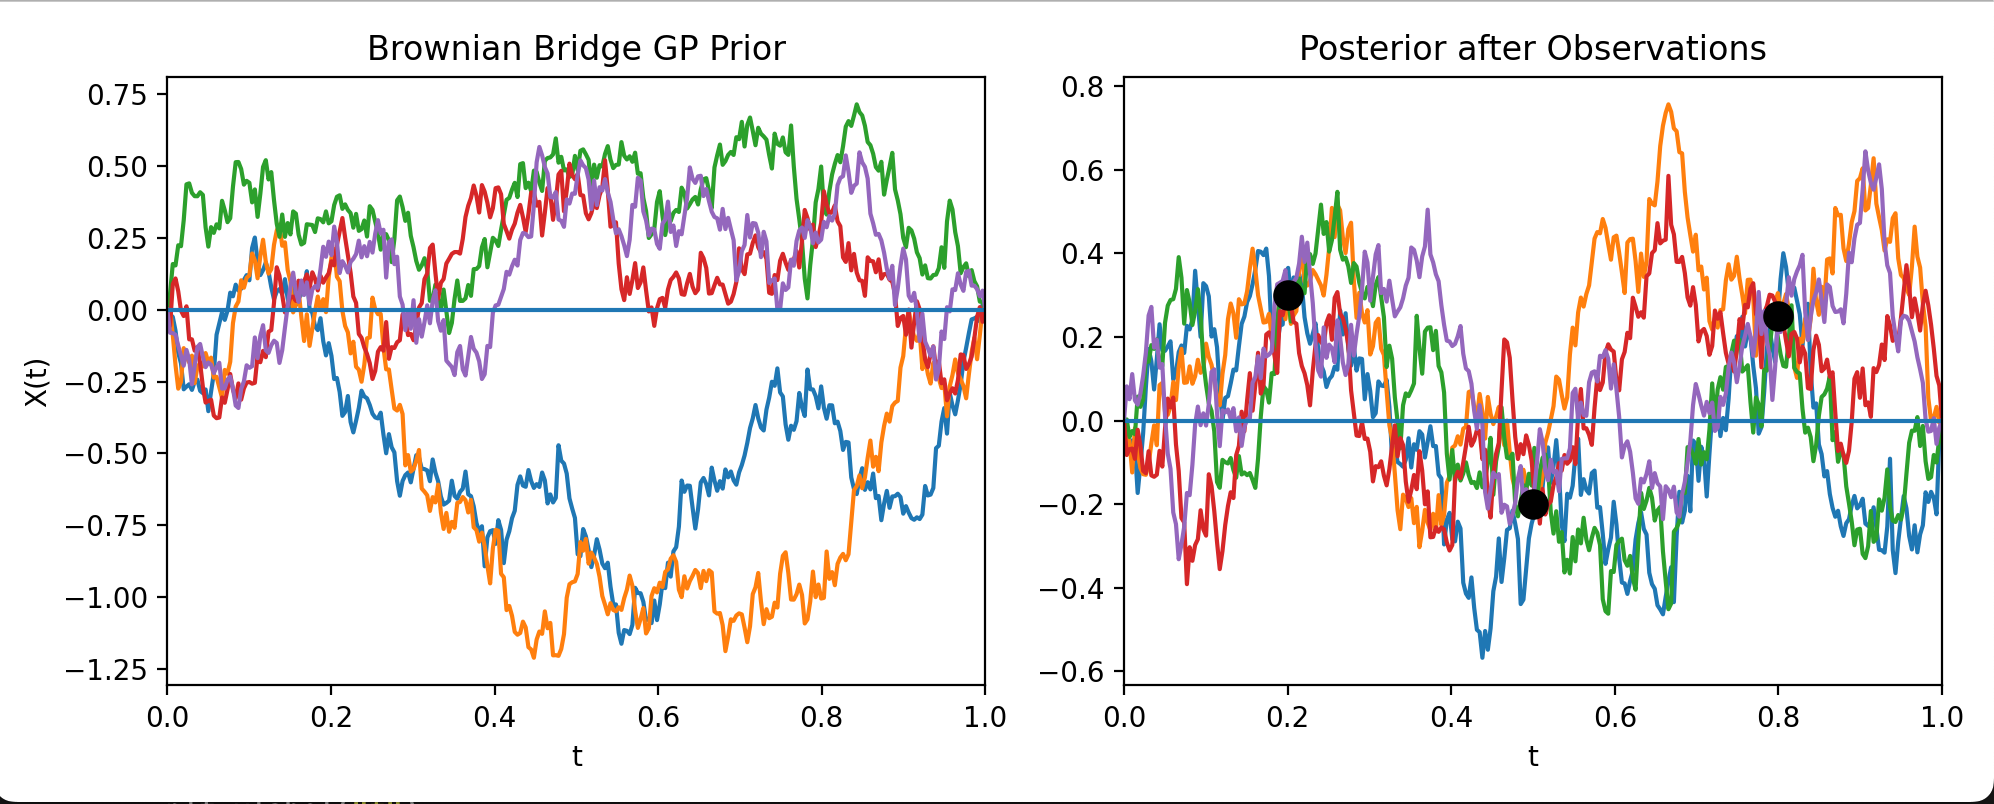
\includegraphics[width=\linewidth]{images/brownian_bridge_gp_prior.png}	
\end{center}
}

\only<2-3>{
\begin{center}
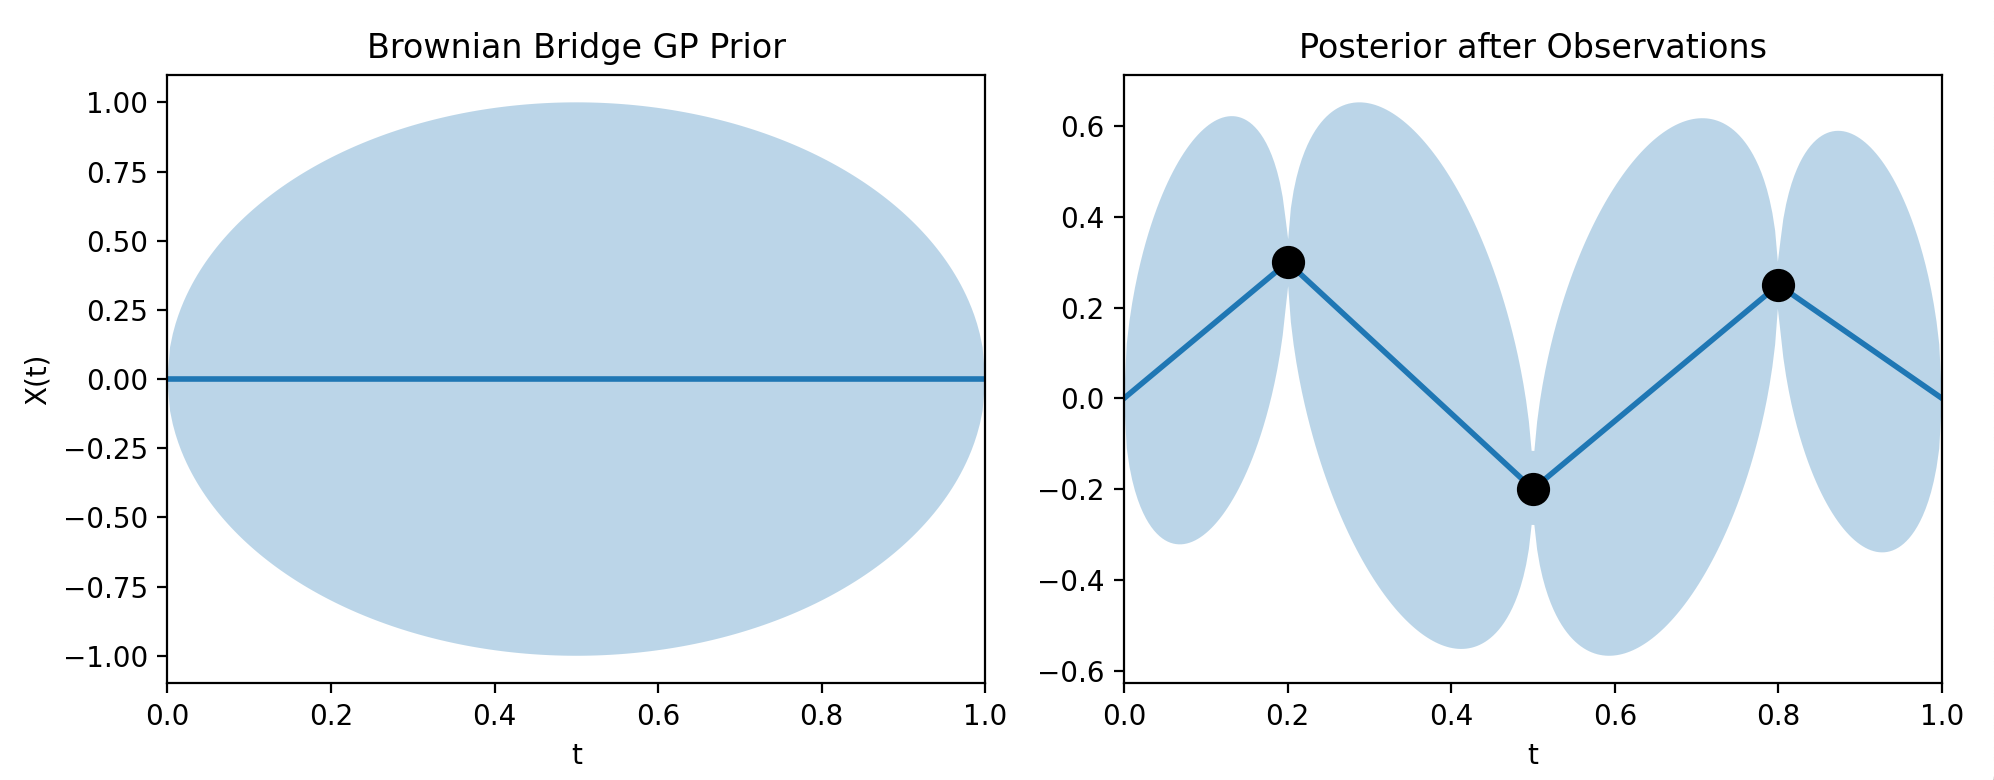
\includegraphics[width=\linewidth]{images/brownian_bridge_gp_prior_2.png}	
\end{center}
}


 
\only<3>{
Examples: 
\begin{itemize}
\item Financial time series with fixed start/end prices
\item Sensor data with boundary constraints
\item Physiological signals aligned to events.
\end{itemize}
}

\end{frame}


\begin{frame}{Brownian Bridge: Use Cases}

\colorbox{green!30}{\textbf{Use Case \#2.}} \textit{Conditional generation and interpolation.}   Can be used to interpolate smoothly and stochastically between two states.


\begin{center}
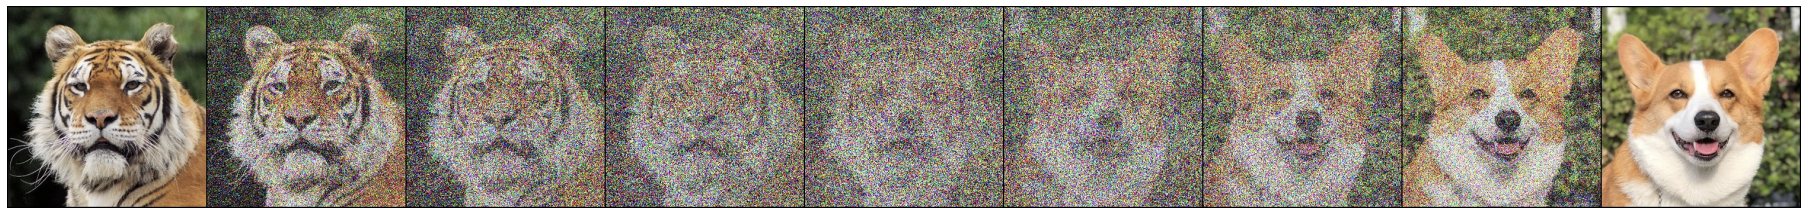
\includegraphics[width=\linewidth]{images/brownian_bridge_interpolation}	
\end{center}
\pause 

Examples: 
\begin{itemize}
\item Image or latent-space interpolation between two images
\item Motion planning with uncertainty
\item Trajectory generation conditioned on start and goal.
\end{itemize}
\bottomtext{\hfill Reference: Zhou et al (2024), Denoising bridge diffusion models, ICLR.}
\end{frame}


\begin{frame}[standout]
Outline for today's material
\begin{itemize}
\item \textbullet \quad Brownian Bridge
\item \textbullet \quad \alert{Diffusion processes}
\end{itemize}

\end{frame}

\begin{frame}{Review: Standard Brownian Motion}

	\fbox{%
	\begin{minipage}{\linewidth}
	%\begin{center}
	\colorbox{blue!30}{\textbf{Definition.}} A \textbf{standard Brownian motion} $\set{W(t): t \geq 0}$ is a stochastic process having
	\begin{itemize}
	\item[(i)] continuous paths,
	\item[(ii)] stationary, independent increments, and
	\item[(iii)] $W(t) \sim N(0,t)$ for all $t \geq 0$.
	\end{itemize} 
	\end{minipage}
}
	
\vfill 
\pause 
\colorbox{green!30}{\textbf{Remark.}} The mean of a standard Brownian motion doesn't change with time, and the variance  increases at rate of 1 unit per second (or whatever unit of time).
\end{frame}

\begin{frame}{Review: Non-Standard Brownian Motion}

	\fbox{%
	\begin{minipage}{\linewidth}
	%\begin{center}
	\colorbox{blue!30}{\textbf{Definition.}} A process $X$ is called a $(\mu, \sigma^2)$ is Brownian motion if it can be written in the form
	\[X(t) = X(0) + \mu t + \sigma W(t), \]
	%\end{center}
	where $W$ is a standard Brownian motion.
	\end{minipage}
	
	}
	
\vfill 
\pause 
\colorbox{green!30}{\textbf{Remark.}}  the mean and variance of a $(\mu, \sigma^2)$ Brownian motion increase at a rate $\mu$ and $\sigma^2$ per second (or whatever unit of time), respectively.

\end{frame}


\begin{frame}{Review: Non-Standard Brownian Motion}

\begin{center}
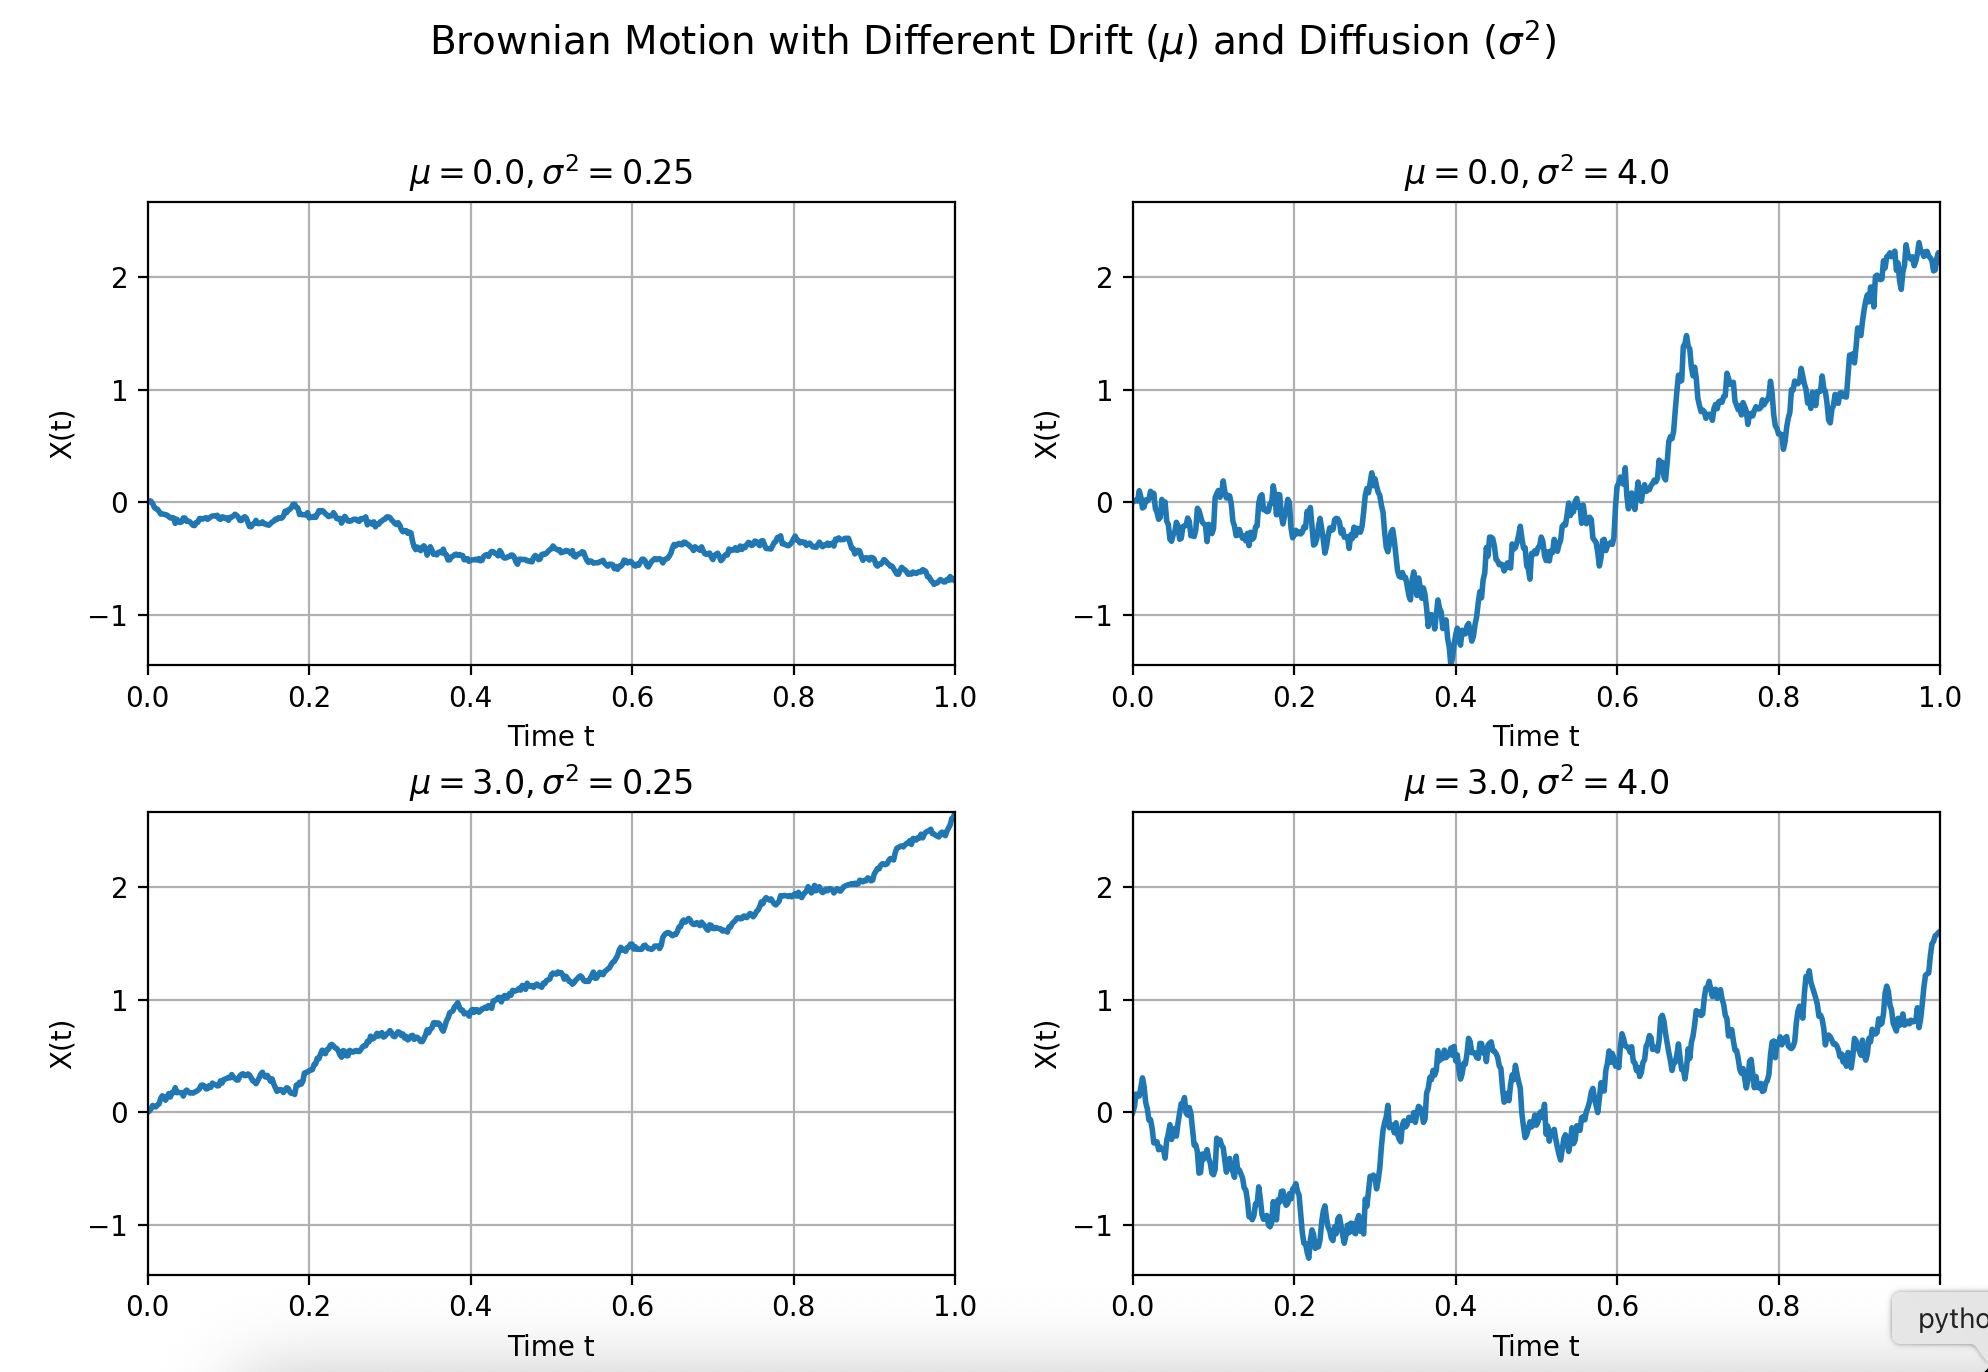
\includegraphics[width=.9\textwidth]{images/brownian_motion_different_drift_and_diffusions.png}	
\end{center}


\end{frame}


\begin{frame}{Diffusion Processes}

\colorbox{red!30}{\textbf{Main Ideas.}}

\begin{itemize}
	\item They are continuous-time, continuous-state Markov processes. \pause 
	\item You can think of them as continuous random variables that evolve over time. \pause 
	\item They are built up from Brownian motion. \pause 
	\begin{itemize}
	\item We specify two functions, $\mu(\cdot)$ and $\sigma^2(\cdot)$.  If the current state is $X_t$, then we (briefly) run a $\bigg( \mu(X_t), \sigma^2(X_t)\bigg)$ Brownian motion.
	\end{itemize}
	\item This is analogous to how we can build up all sorts of differentiable functions (e.g. the exponential function) from lines.
\end{itemize}
	
\end{frame}

\begin{frame}{A definition of a diffusion process}


	\fbox{%
	\begin{minipage}{\linewidth}
	%\begin{center}
	\colorbox{blue!30}{\textbf{Definition.}} A process $(X_t)$ is called a diffusion process if it has these properties
	\begin{enumerate}
		\item The time variable $t$ is continuous.
		\item It is a Markov process.  (This means that $X_{t_0}$ determines the distribution of $X_t$ for $t>t_0$ ``completely.'')
		\item $X_t$ is a continuous function of $t$. 
	\end{enumerate}
	\end{minipage}
	
	}
	
\bottomtext{\hfill Reference: Johnathan Goodman, course notes.}	
\end{frame}




\begin{frame}{Discretization of a diffusion process}

Let $\Delta X = X_{t + \Delta t} - X_t$ be a small change in the diffusion process. Then per Chang pp.180, we have
	\begin{align*}
	 \Delta X = \mu(X_t) \Delta t + \sigma(X_t) \, \sqrt{\Delta t} \, Z  \qquad Z, \sim N(0,1)
	\end{align*}
		
\end{frame}



\begin{frame}{Examples of Diffusion Processes}

\begin{itemize}
	\item \textit{Brownian Motion} \pause 
	\item \textit{Brownian Bridges} \pause 
	\item \textit{Geometric Brownian Motion} - a model for stocks (the ``returns'', or ratios, are independent over non-overlapping intervals) \pause 
	\item \textit{Ornstein-Uhlenbeck Process} - a mean reverting process \pause 
	\item \textit{Wright-Fisher Process} - a process with two absorbing states (can model allele frequency in genetics)
\end{itemize}
	
See Chang Sec 6.2 for pictures and further details.
\end{frame}


\begin{frame}{Random Groups}

\begin{columns}
\begin{column}{0.33\textwidth}
Aubrey Williams: 4 \\ 
Austin Barton : 6 \\ 
Blake Sigmundstad: 6 \\ 
Diego Moylan: 5 \\ 
Dillon Shaffer: 8 \\ 
Ismoiljon Muzaffarov: 2 \\ 
Jacob Tanner: 4 \\\end{column}
\begin{column}{0.33\textwidth}
Josh Stoneback: 4 \\ 
Joshua Bowen: 1 \\ 
Joshua Culwell: 3 \\ 
Laura Banaszewski: 1 \\ 
Lina Hammel: 7 \\ 
Logan Racz: 7 \\\end{column}
\begin{column}{0.33\textwidth}
Matt Hall: 5 \\ 
Micah Miller: 3 \\ 
Mike Kadoshnikov: 1 \\ 
Owen Cool: 2 \\ 
Racquel Bowen: 3 \\ 
Samuel Mocabee: 2 \\ 
Tatiana Kirillova: 8 \\\end{column}
\end{columns}
\end{frame}



\begin{frame}{Group exercises - Problem Set 12}
\footnotesize  
\begin{enumerate}
	\item (Chang Sec 5.6)  \textbf{Brownian Bridge.} Verify that the below is an easy way to manufacture a Brownian bridge from standard Brownian motion:
	\[ X(t) = W(t)-t W(1), \qquad \text{for } 0 \leq t \leq 1.\]
	\fbox{%
	\begin{minipage}{\linewidth}
	%\begin{center}
	\colorbox{blue!30}{\textbf{Definition.}} A standard Brownian Bridge is a Gaussian process $X$ with continuous paths, mean 0, and covariance function $\Cov(X_s, X_t)=s(1-t)$ for $0 \leq s \leq t \leq 1$.
	%\end{center}
	\end{minipage}
	
	}
\item (Chang Sec 6.1) \textbf{Discretized Diffusion.} Let $\Delta X = X_{t + \Delta t} - X_t$ be a small change in the diffusion process. Then per Chang pp.180, we have
	\begin{align*}
	 \Delta X = \mu(X_t) \Delta t + \sigma(X_t) \, \sqrt{\Delta t} \, Z  \qquad Z, \sim N(0,1)
	\end{align*}
	%
	Show that as $\Delta t \downarrow 0$.
	\begin{align*}
	\E[\Delta X \mid X(t)=x] = \mu(x) \Delta t + o(\Delta t)\\	
	\E[(\Delta X)^2 \mid X(t)=x] = \sigma^2(x) \Delta t + o(\Delta t)
	\end{align*}

	\fbox{%
	\begin{minipage}{\linewidth}
	%\begin{center}
	\colorbox{blue!30}{\textbf{Definition.}} Let $f(x)$ and $g(x)$ be functions defined on some neighborhood of $x_0$. We write
	$f(x) = o(g(x))$ as $x \to x_0$ if 
	\[
	\lim_{x \to x_0} \frac{f(x)}{g(x)} = 0.
	\]
Equivalently, $f(x)$ becomes negligible relative to $g(x)$ as $x$ approaches $x_0$.
	%\end{center}
	\end{minipage}
	
	}	 
\end{enumerate}


\end{frame}


\end{document}
